\documentclass[border=10pt]{standalone}
\usepackage{tikz}
\usetikzlibrary{shapes}

\begin{document}
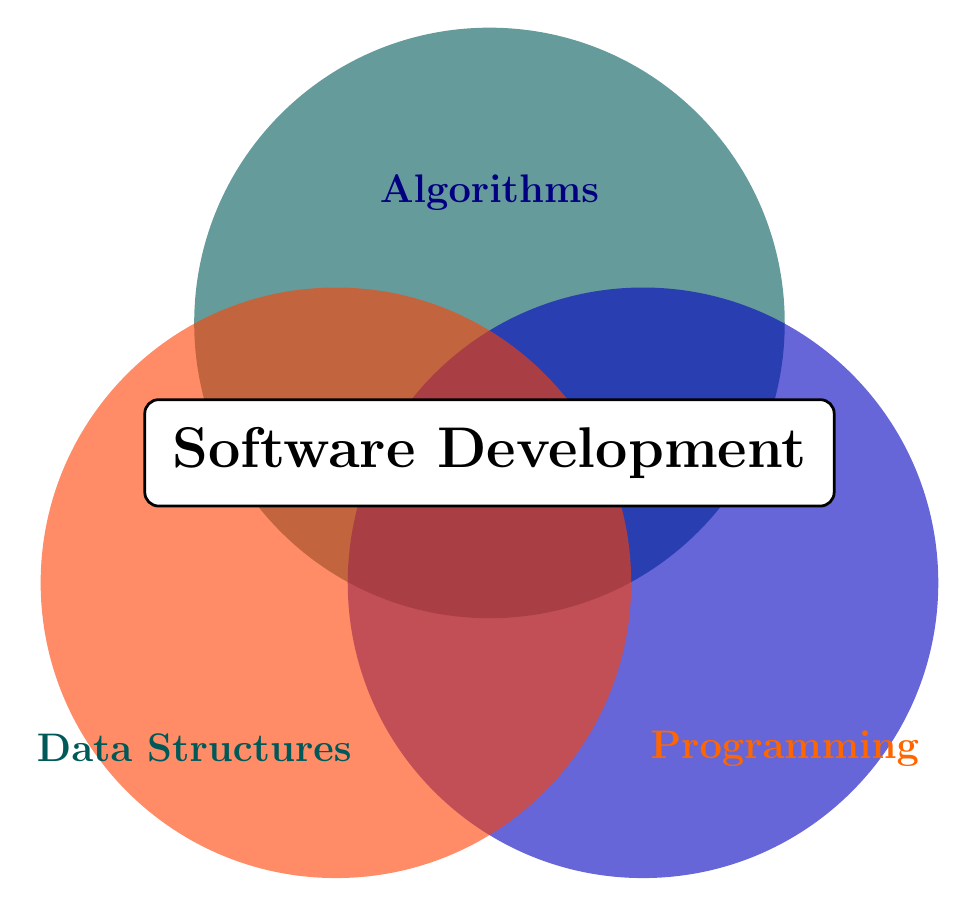
\begin{tikzpicture}[scale=1.5]
    % Define circle parameters
    \def\radius{2.5}
    \def\offsetx{1.3}
    \def\offsety{1.1}
    
    % Draw circles with transparency
    \begin{scope}[opacity=0.6]
        % Top circle - Algorithms (teal)
        \fill[teal!70!black] (0, \offsety) circle (\radius);
        
        % Bottom-right circle - Programming (blue-purple)
        \fill[blue!75!black] (\offsetx, -\offsety) circle (\radius);
        
        % Bottom-left circle - Data Structures (coral)
        \fill[orange!50!red] (-\offsetx, -\offsety) circle (\radius);
    \end{scope}
    
    % Add labels for each circle
    \node[font=\Large\bfseries, color=blue!50!black] at (0, 2.2) {Algorithms};
    \node[font=\Large\bfseries, color=teal!70!black] at (-2.5, -2.5) {Data Structures};
    \node[font=\Large\bfseries, color=orange!80!red] at (2.5, -2.5) {Programming};
    
    % Central label box
    \node[rectangle, rounded corners=5pt, fill=white, draw=black, line width=1pt, 
          font=\huge\bfseries, inner sep=10pt] at (0, 0) {Software Development};
    
\end{tikzpicture}
\end{document}
